% ----------------------------------------------------------------------
%  Pracovní úkoly
% ----------------------------------------------------------------------
\section{Pracovní úkoly}

\begin{enumerate}
\item Pro tři vodorovné trubice s různými poloměry kruhového průřezu, které jsou opatřeny manometry, změřte závislost objemového průtoku Qv na úbytku statického tlaku \(\Delta p\) na vyšetřované délce trubice l ve směru proudění.

\item Sestrojte graf závislosti \(Qv = Qv(p).\)

\item Ze směrnice závislosti \(Qv = Qv(p)\) v oblasti laminárního proudění určete poloměr trubice.

\item Upravený poloměr dosaďte do vztahů pro výpočet Re a k.

\item Sestrojte graf závislosti k = k(Re), kde k je součinitel odporu trubice a Re je Reynoldsovo číslo. Do grafu vyneste teoretickou závislost pro laminární i turbulentní proudění.
\end{enumerate}

% ----------------------------------------------------------------------
%  Teoretická část
% ----------------------------------------------------------------------
\section{Teoretická část}

    Pro studium závislosti objemového průtoku \(Q_V\) na úbytku statického tlaku \(\Delta p\) použijeme aparaturu znázorněnou na obr. \ref{fig:schema}. Díky této závislosti určíme i oblasti laminárního a turbulentního proudění. Změnou rychlosti proudění vody v trubici s milimetrovou stupnicí se mění výška hladiny v manometru. Úbytek statického tlaku je dán vztahem

    \begin{equation}
        \Delta p = h\rho g,
    \end{equation}

    kde \(\rho\) je hustota kapaliny a \(g\) je místní tíhové zrychlení.

    \begin{figure}[h]
        \centering
        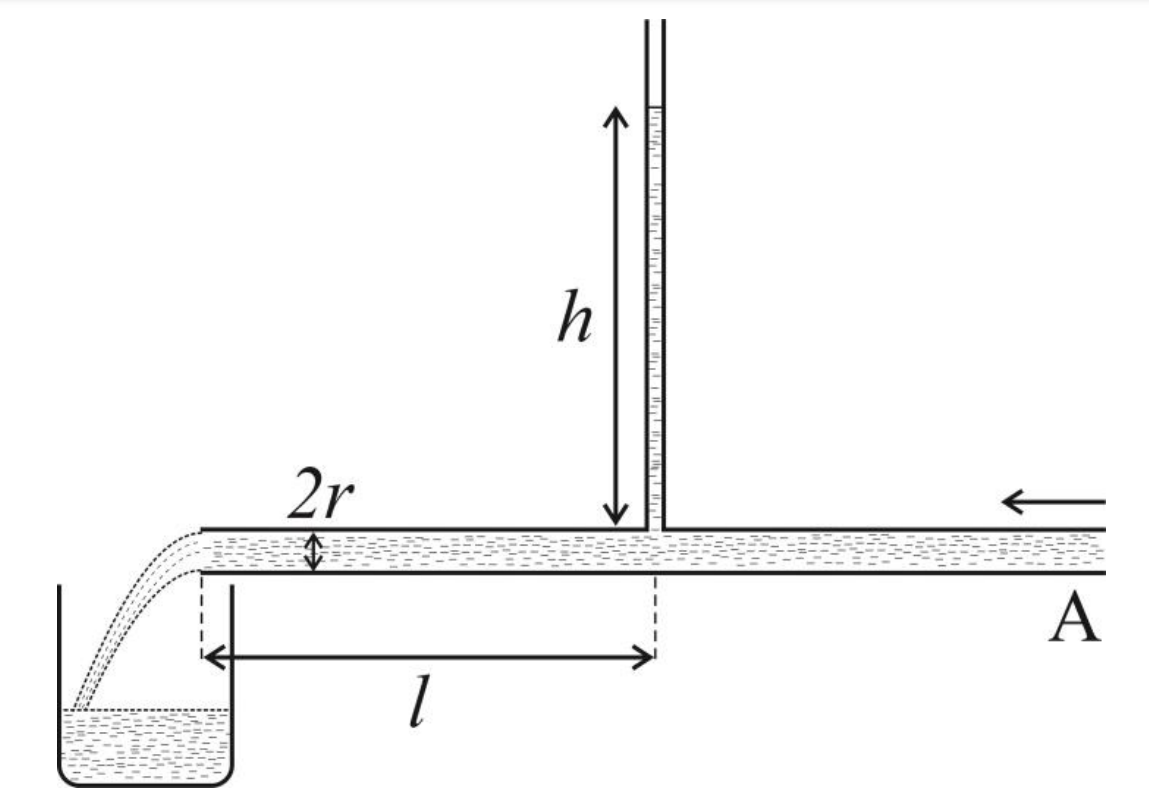
\includegraphics[width=0.5\linewidth]{01 - Studium proudění viskózní kapaliny trubicemi kruhového průřezu//Protokol//img/Schéma.png}
        \caption{Schéma zařízení.}
        \label{fig:schema}
    \end{figure}

    Objemový průtok je dán vztahem

    \begin{equation}
        Q_V = \frac{V}{t},
    \end{equation}

    kde \(V\) je objem kapaliny proteklé trubicí za čas \(t\).

    V oblasti laminárního proudění pro objemový průtok platí Poiseuillova rovnice

    \begin{equation}
        Q_V = \frac{\pi r^4}{8\eta l}\Delta p,
    \end{equation}

    kde \(r\) je vnitřní poloměr, \(l\) délka trubice a \(\eta\) dynamická viskozita proudící kapaliny.

    Proudění je laminární pokud nepřekročí kritickou hodnotu Reynoldsova čísla

    \begin{equation}
        Re = \frac{r\rho v_s}{\eta},
    \end{equation}

    kde \(v_s\) je střední rychlost proudění v trubici. Tato oblast je však určena pouze přibližně.

    \(v_s\) lze vyjádřit jako

    \begin{equation}
        v_s = \frac{Q_V}{\pi r^2}
    \end{equation}

    Úpravou lze součinitel odporu trubice \(k\) na základě naměřených hodnot vyjádřit jako

    \begin{equation}
        k = \frac{2r^5\pi^2\Delta p}{\rho Q_V^2 l}
    \end{equation}

    Pro laminární proudění platí teoretický vztah

    \begin{equation}
        k = \frac{16}{Re},
    \end{equation}

    kde k je součinitel odporu trubice.

    Pro trubice s hladkými stěnami lze použít v případě turbulentního proudění lze použít vztah:

    \begin{equation}
        k \approx \frac{0,133}{\sqrt[4]{Re}}
    \end{equation}
% ----------------------------------------------------------------------
%  Výsledky a zpracování měření
% ----------------------------------------------------------------------
\section{Výsledky a zpracování měření}

\subsection{Laboratorní podmínky}

    Měření bylo prováděno za laboratorních podmínek uvedených v tabulce \ref{tab:lab_pod}. Pro naše měření je ale důležité, aby hodnoty (jako například teplota vody procházející  trubicí) byly co možná nejvíce podobné po celou dobu.

    \begin{table}[h]
        \centering
        \caption{Laboratorní podmínky}
        \label{tab:lab_pod}
        \begin{tabular}{|c|c|c|} 
        \hline
            t / °C & p / hPa & vlhkost / \%RH  \\ 
        \hline
            22,9(40)   & 977,2(20)   & 34,7(25)            \\
        \hline
        \end{tabular}
    \end{table}

\subsection{Rozměry trubic}

    Vnitřní průměry trubic byly měřeny pomocí plastového posuvného měřidla. Udávaná přesnost je 0,05 mm, protože je ale měřidlo vyrobené z plastu a již lehce opotřebované, ve skutečnosti je přesnost nižší. V tabulce \ref{tab:prumery} jsou uvedeny výsledné průměry pro každou trubici (A, B a C). Každá trubice byla změřena třikrát.

    \begin{table}[h]
        \centering
        \caption{Vnitřní průměry trubic}
        \label{tab:prumery}
        \begin{tabular}{|c|c|c|c|} 
        \hline
            číslo měření & d_A / mm & d_B / mm & d_C / mm  \\ 
        \hline
            1            & 2,1(5)    & 2,7(5)    & 3,1(5)   \\
            2            & 2,1(5)    & 2,5(5)    & 3,0(5)   \\
            3            & 2,1(5)    & 2,7(5)    & 3,0(5)   \\ 
        \hline
            aritmetický průměr   & 2,1       & 2,6       & 3,0         \\
            standardní odchylka        & 0       & 0,1       & 0,1     \\
        \hline
        \end{tabular}
    \end{table}

    Vzdálenosti \(l\) každé trubice jsou uvedeny v tabulce \ref{tab:délky}. Tato vzdálenost byla změřena svinovacím metrem s přesností 0,5 mm.

    \begin{table}[h]
        \centering
        \caption{Délky trubic}
        \label{tab:délky}
        \begin{tabular}{|c|c|c|c|} 
        \hline
            číslo měření & d_A / mm & d_B / mm & d_C / mm  \\ 
        \hline
            1            & 251(5)    & 250(5)    & 202(5)   \\
            2            & 251(5)    & 250(5)    & 202(5)   \\
            3            & 251(5)    & 250(5)    & 202(5)   \\ 
        \hline
            výsledek     & 251(5)    & 250(5)    & 202(5)   \\
        \hline
        \end{tabular}
    \end{table}
\newpage

\subsection{Teplota vody}

    Teplota vody byla změřena rtuťovým teploměrem třikrát - na začátku, v průběhu a na konci celého měření. Voda do trubice přitéká ze zásobníku na vodu, který je umístěn nad aparaturou. Je žádoucí, aby voda přitékala stále se stejnou teplotou, ale kvůli okolní teplotě lze předpokládat, že se v průběhu času postupně ohřívá.

    \begin{table}[h]
        \centering
        \caption{Teploty vody}
        \label{tab:teploty_vody}
        \begin{tabular}{|c|} 
        \hline
            t / °C   \\ 
        \hline
            21,8(5)  \\
            22,1(5)  \\
            22,2(5)  \\
        \hline
        \end{tabular}
    \end{table}

    Na základě této teploty lze určit podle tabulek hustotu vody, která je 997,818 \SI{}{\kg\water\per\m\cubed\air}. Pro naše měření bude však pracovat s hodnotou 997(1) \SI{}{\kg\water\per\m\cubed\air}.

\subsection{Závislost objemového průtoku na úbytku tlaku}

    Závislost průtoku na tlaku byla měřena pomocí odměrného válce a ručních stopek. Množství vody a tedy její rychlost a změna tlaku byla regulována otočným kohoutem. Na začátku měření trubice byla stupnice manometru přibližně rozdělena do oblastí, kde dochází k laminárnímu proudění a kde ne. Díky to bylo možné naplánovat jednotlivá měření pro dostatek dat v laminární oblasti.

    V určité výšce manometru byl nastaven určitý tlak a poté změřen objem kapaliny proteklý trubicí za čas. V oblasti turbulentního proudění hladina vody v manometru neustále oscilovala, proto byla výška v tomto případě nastavena tak, aby hladina oscilovala kolem měřené hodnoty. Díky poměrně přesné milimetrové stupnici manometru byla nejistota výšky \(h\) odhadnuta na 0,05 cm ve stabilní oblasti laminárního proudění, v ostatních případech na 0,2 cm. Čas byl měřen pomocí stopek, kde počítáme s odchylkou reakční doby člověka, která je rovna přibližně 0,2 s. Nejistota měření objemu byla určena 10 ml pro trubici C, pro trubici A a B 2 ml. Tato chyba u trubice C je dána použitím méně přesného odměrného válce.
    
    Chyba \(\Delta p\) byla vypočtena pomocí metody přenosu chyb podle

    \begin{equation}
        \frac{\sigma_\Delta_p}{\Delta_p} = \sqrt{(\frac{\sigma_h}{h})^2 + (\frac{\sigma_\rho}{\rho})^2}
    \end{equation}

    Chyba objemového průtoku \(Q_V\) byla vypočtena také podle metody přenosu chyb jako

    \begin{equation}
        \frac{\sigma_Q__V}{\frac{V}{t}} = \sqrt{(\frac{\sigma_V}{V})^2+(\frac{\sigma_t}{t})^2}
    \end{equation}

\newpage

    \begin{table}[h]
        \centering
        \caption{Trubice A}
        \label{tab:trubice A}
        \begin{tabular}{|c|c|c|c|c|}
        \hline
            h / cm   & V / ml  & t / s      & ∆p / Pa & Q_V / 10^{-6} \frac{m^3}{s}  \\ 
        \hline
            11(0.05)     & 200(2)    & 100,1(2) & 1077(5)   & 2,0(0,2)     \\
            12(0.05)     & 85(2)     & 37,3(2)  & 1175(5)   & 2,3(0,5)     \\
            14(0.05)     & 100(2)    & 36,5(2)  & 1370(5)   & 2,7(0,6)     \\
            15(0.05)     & 115(2)    & 39,3(2)  & 1468(5)   & 2,9(0,5)     \\
            16(0.05)     & 135(2)    & 41,7(2)  & 1566(5)   & 3,2(0,5)     \\
            17(0.05)     & 200(2)    & 60,7(2)  & 1664(5)   & 3,3(0,3)     \\
            18(0.05)     & 200(2)    & 57,2(2)  & 1762(5)   & 3,5(0,4)     \\
            20(0.05)     & 175(2)    & 49,8(2)  & 1958(5)   & 3,5(0,4)     \\
        \hline
        \end{tabular}
    \end{table}

    \begin{table}[h]
        \centering
        \caption{Trubice B}
        \label{tab:trubice B}
        \begin{tabular}{|c|c|c|c|c|} 
        \hline
            h / cm & V / ml & t / s & p / Pa & Q_V / 10^{-6} \frac{m^3}{s}    \\ 
        \hline
            7(0,05)      & 205(2)    & 47,5(2)  & 685(5)    & 4,3(0,5)  \\
            8(0,05)      & 205(2)    & 42,6(2)  & 783(5)    & 4,8(0,5)  \\
            9(0,05)      & 195(2)    & 37,7(2)  & 881(5)    & 5,2(0,6)  \\
            10(0,05)     & 200(2)    & 34,4(2)  & 979(5)    & 5,8(0,7)  \\
            11(0,05)     & 205(2)    & 34,4(2)  & 1077(5)   & 6,0(0,7)  \\
            12(0,05)     & 205(2)    & 31,9(2)  & 1175(5)   & 6,4(0,7)  \\
            13(0,2)     & 230(2)    & 34,5(2)  & 1273(20)   & 6,7(0,7)  \\
            14(0,2)     & 200(2)    & 27,5(2)  & 1370(20)   & 7,3(0,9)  \\
            15(0,2)     & 200(2)    & 26,4(2)  & 1468(20)   & 7,6(1)  \\
            16(0,2)     & 195(2)    & 24,9(2)  & 1566(20)   & 7,8(1)  \\
            17(0,2)     & 195(2)    & 24,5(2)  & 1664(20)   & 7,9(1)  \\
        \hline
        \end{tabular}
    \end{table}

    \begin{table}[h]
        \centering
        \caption{Trubice C}
        \label{tab:trubice C}
        \begin{tabular}{|c|c|c|c|c|}
        \hline
            h / cm   & V / ml  & t / s      & ∆p / Pa & Q_V / 10^{-6} \frac{m^3}{s}  \\ 
        \hline
            23(0,2) & 200(10) & 20,7(2)  & 2251(20)  & 9,7(5)             \\
            22(0,2) & 200(10) & 21,5(2)  & 2154(20)  & 9,3(5)             \\
            21(0,2) & 200(10) & 21,6(2)  & 2056(20)  & 9,3(5)             \\
            20(0,2) & 200(10) & 22,4(2)  & 1958(20)  & 8,9(5)             \\
            19(0,2) & 200(10) & 23,3(2)  & 1860(20)  & 8,6(4)             \\
            18(0,2) & 200(10) & 23,8(2)  & 1762(20)  & 8,4(4)             \\
            17(0,2) & 200(10) & 24,6(2)  & 1664(20)  & 8,1(4)             \\
            16(0,2) & 200(10) & 25,2(2)  & 1566(20)  & 7,9(4)             \\
            15(0,2) & 200(10) & 26,9(2)  & 1468(20)  & 7,4(4)             \\
            14(0,2) & 200(10) & 27,0(2)  & 1370(20)  & 7,4(4)             \\
            13(0,2) & 200(10) & 28,1(2)  & 1273(20)  & 7,1(4)             \\
            12(0,2) & 200(10) & 28,0(2)  & 1175(20)  & 7,1(4)             \\
            11(0,2) & 200(10) & 28,4(2)  & 1077(20)  & 7,0(4)             \\
            10(0,2) & 200(10) & 29,1(2)  & 979(20)   & 6,9(3)             \\
            9(0,05)  & 200(10) & 29,2(2)  & 881(5)   & 6,8(3)             \\
            8(0,05)  & 200(10) & 31,0(2)  & 783(5)   & 6,5(3)             \\
            7(0,05)  & 200(10) & 33,4(2)  & 685(5)   & 6,0(3)             \\
            6(0,05)  & 200(10) & 37,8(2)  & 587(5)   & 5,3(3)             \\
            5(0,05)  & 200(10) & 42,7(2)  & 489(5)   & 4,7(2)             \\
            4(0,05)  & 200(10) & 51,1(2)  & 392(5)   & 3,9(2)             \\
            3(0,05)  & 200(10) & 69,8(2)  & 294(5)   & 2,7(1)             \\
            2(0,05)  & 200(10) & 105,8(2) & 196(5)   & 1,9(1)             \\
        \hline
        \end{tabular}
    \end{table}

\newpage

\begin{figure}[h]
    \centering
    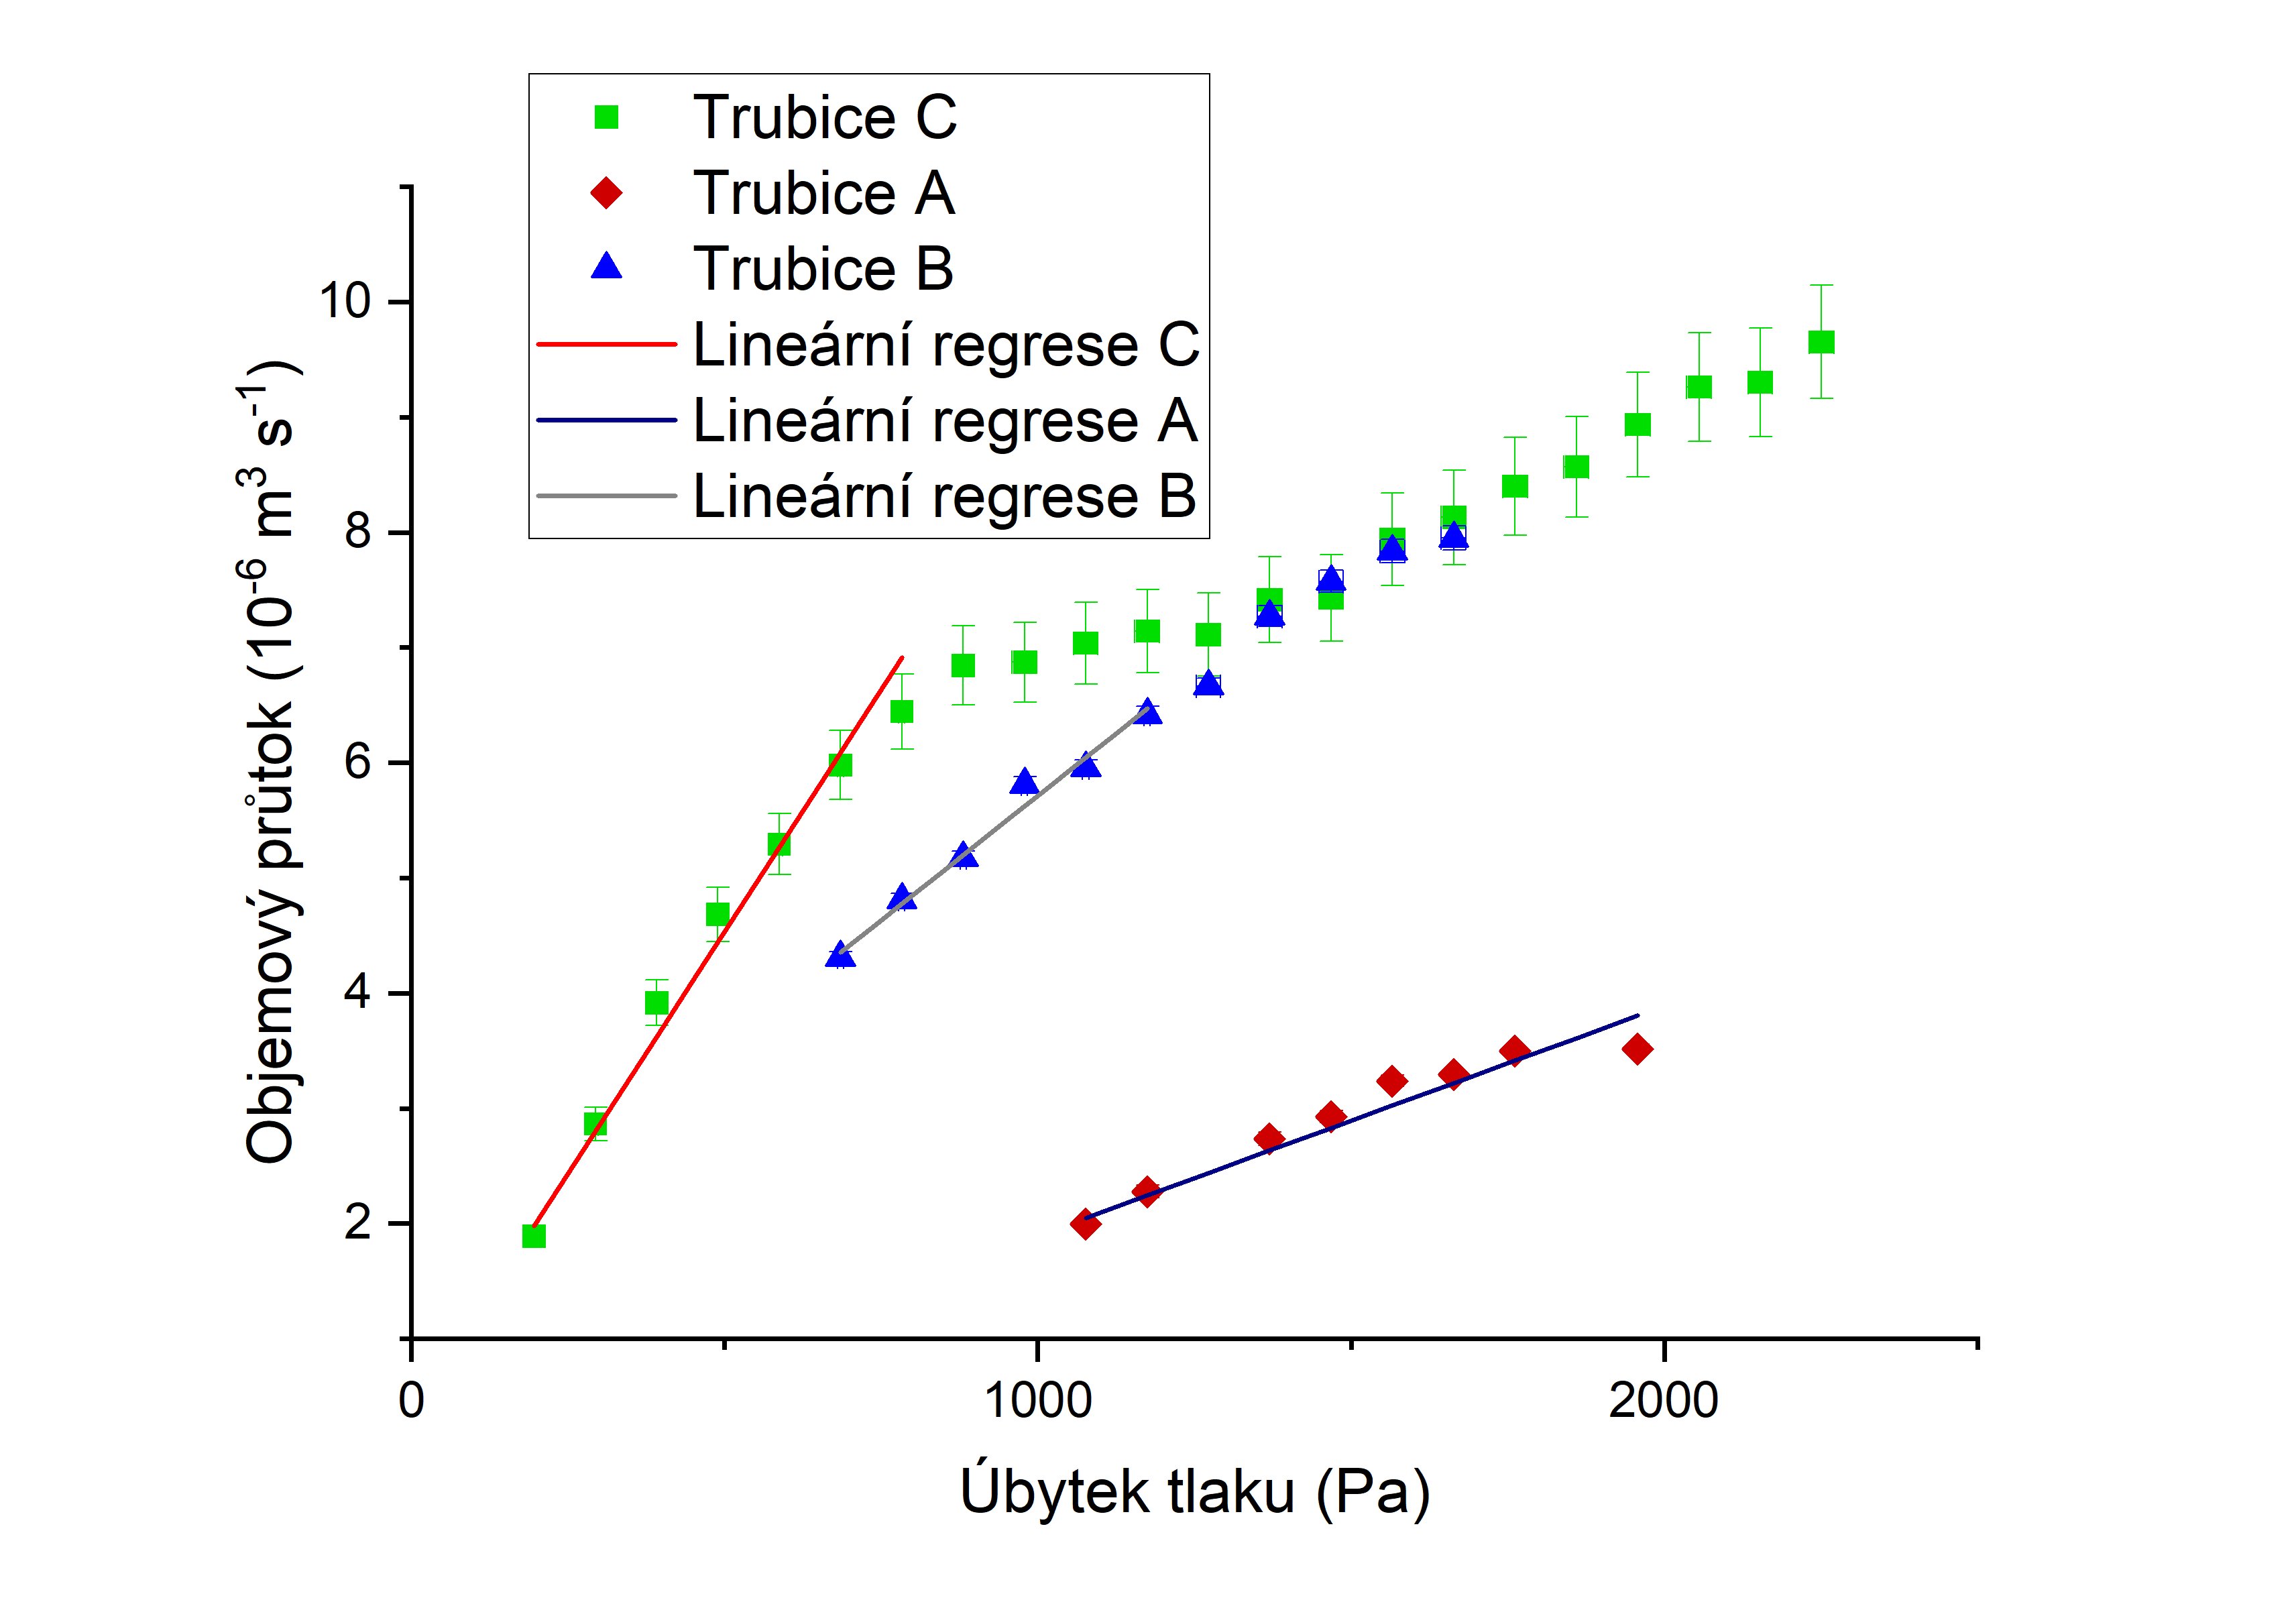
\includegraphics[width=0.65\linewidth]{01 - Studium proudění viskózní kapaliny trubicemi kruhového průřezu//Protokol//img/Trubice A, B a C.png}
    \caption{Graf závislosti objemového průtoku na poklesu tlaku trubic}
    \label{fig:graf trubic}
\end{figure}

\newpage

    U závislosti každé trubice byla určena lineární regrese v oblastech laminárního proudění. Tento fit je vážen nejistotou jednotlivých měření. Je zde určena i standardní chyba, která byla škálována s druhou odmocninou redukovaného chi-kvadrátu.

    Podle vztahu (3) pro směrnici grafu platí

    \begin{equation}
        f = \frac{\pi r^4}{8 \eta l}
    \end{equation}

    dynamická viskozita vody má při naší teplotě hodnotu

    \begin{equation}
        \eta = 950 \cdot 10^{-6} Pa \cdot s
    \end{equation}

    Jednotlivé směrnice závislostí jsou

    \begin{table}[h]
        \centering
        \begin{tabular}{|c|c|} 
        \hline
            Trubice & Směrnice se standardní chybou / kg^{-1} m^{4} s  \\ 
        \hline
            A       & (2,0 \pm 0,2) \cdot 10^{-9}                                \\
            B       & (4,3 \pm 0,2) \cdot 10^{-9}                                \\
            C       & (8,4 \pm 0,4) \cdot 10^{-9}                                \\
        \hline
        \end{tabular}
    \end{table}

    Ze vztahu (9) lze odvodit rovnost pro výpočet poloměru trubice ze směrnice

    \begin{equation}
        r = \sqrt[4]{\frac{8\eta fl}{\pi}}
    \end{equation}

    Poté můžeme porovnat výsledky průměry trubic změřené plastovým posuvným měřidlem a výpočtem ze směrnice. Rovnost (11) nám dává pouze poloměr, proto musíme výsledek ještě vynásobit dvěma.

    \begin{table}[h]
        \centering
        \begin{tabular}{|c|c|c|} 
        \hline
            Trubice & Vnitřní průměr podle měřidla / mm & Vnitřní průměr ze směrnice / mm  \\ 
        \hline
            A       & 2,1                           & 2,1                              \\
            B       & 2,6                           & 2,5                              \\
            C       & 3,0                           & 2,8                              \\
        \hline
        \end{tabular}
    \end{table}

\subsection{Součinitel odporu trubice}

    Nyní dosadíme upravený poloměr do vztahu (4) pro výpočet Reynoldsova čísla (6) pro součinitel odporu trubice. Tyto hodnoty pak porovnáme s teoretickou závislostí (7).

    \begin{figure}[h]
        \centering
        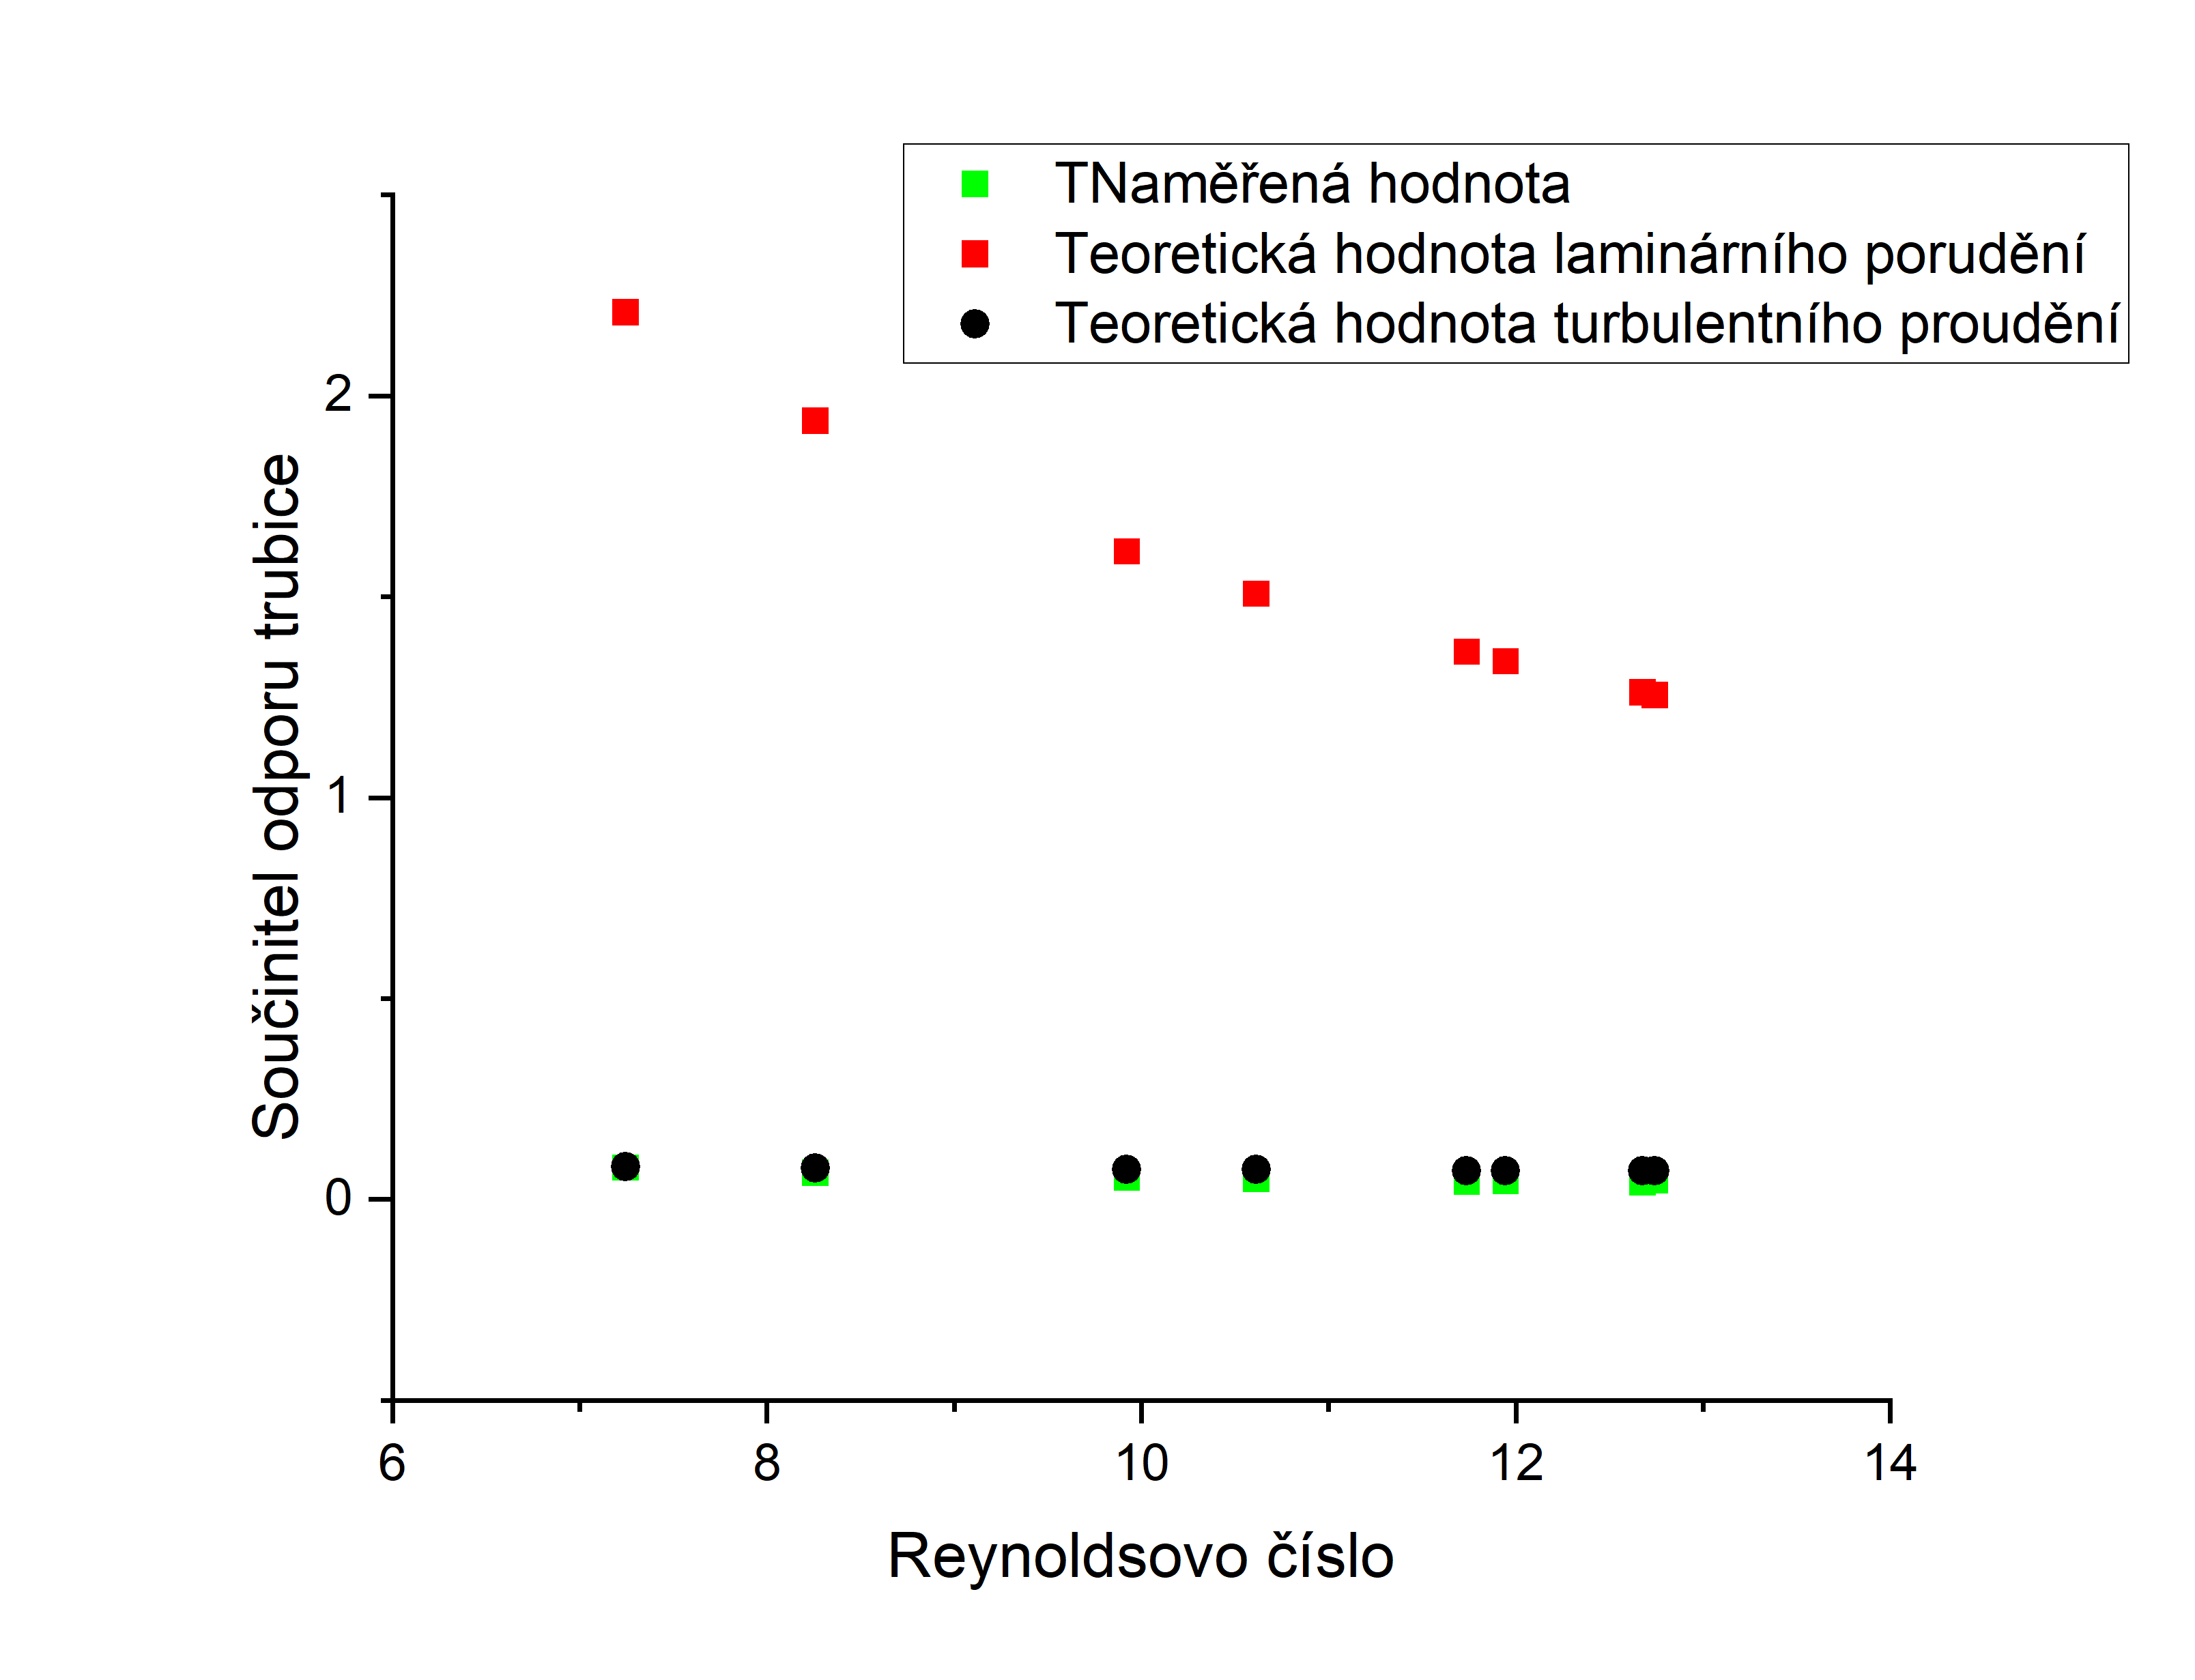
\includegraphics[width=0.6\linewidth]{01 - Studium proudění viskózní kapaliny trubicemi kruhového průřezu//Protokol//img/Re(k) A.png}
        \caption{Závislost součinitele odporu trubice A na Reynoldsově čísle}
        \label{fig:Re(k) A}
    \end{figure}    

    \begin{figure}[h]
        \centering
        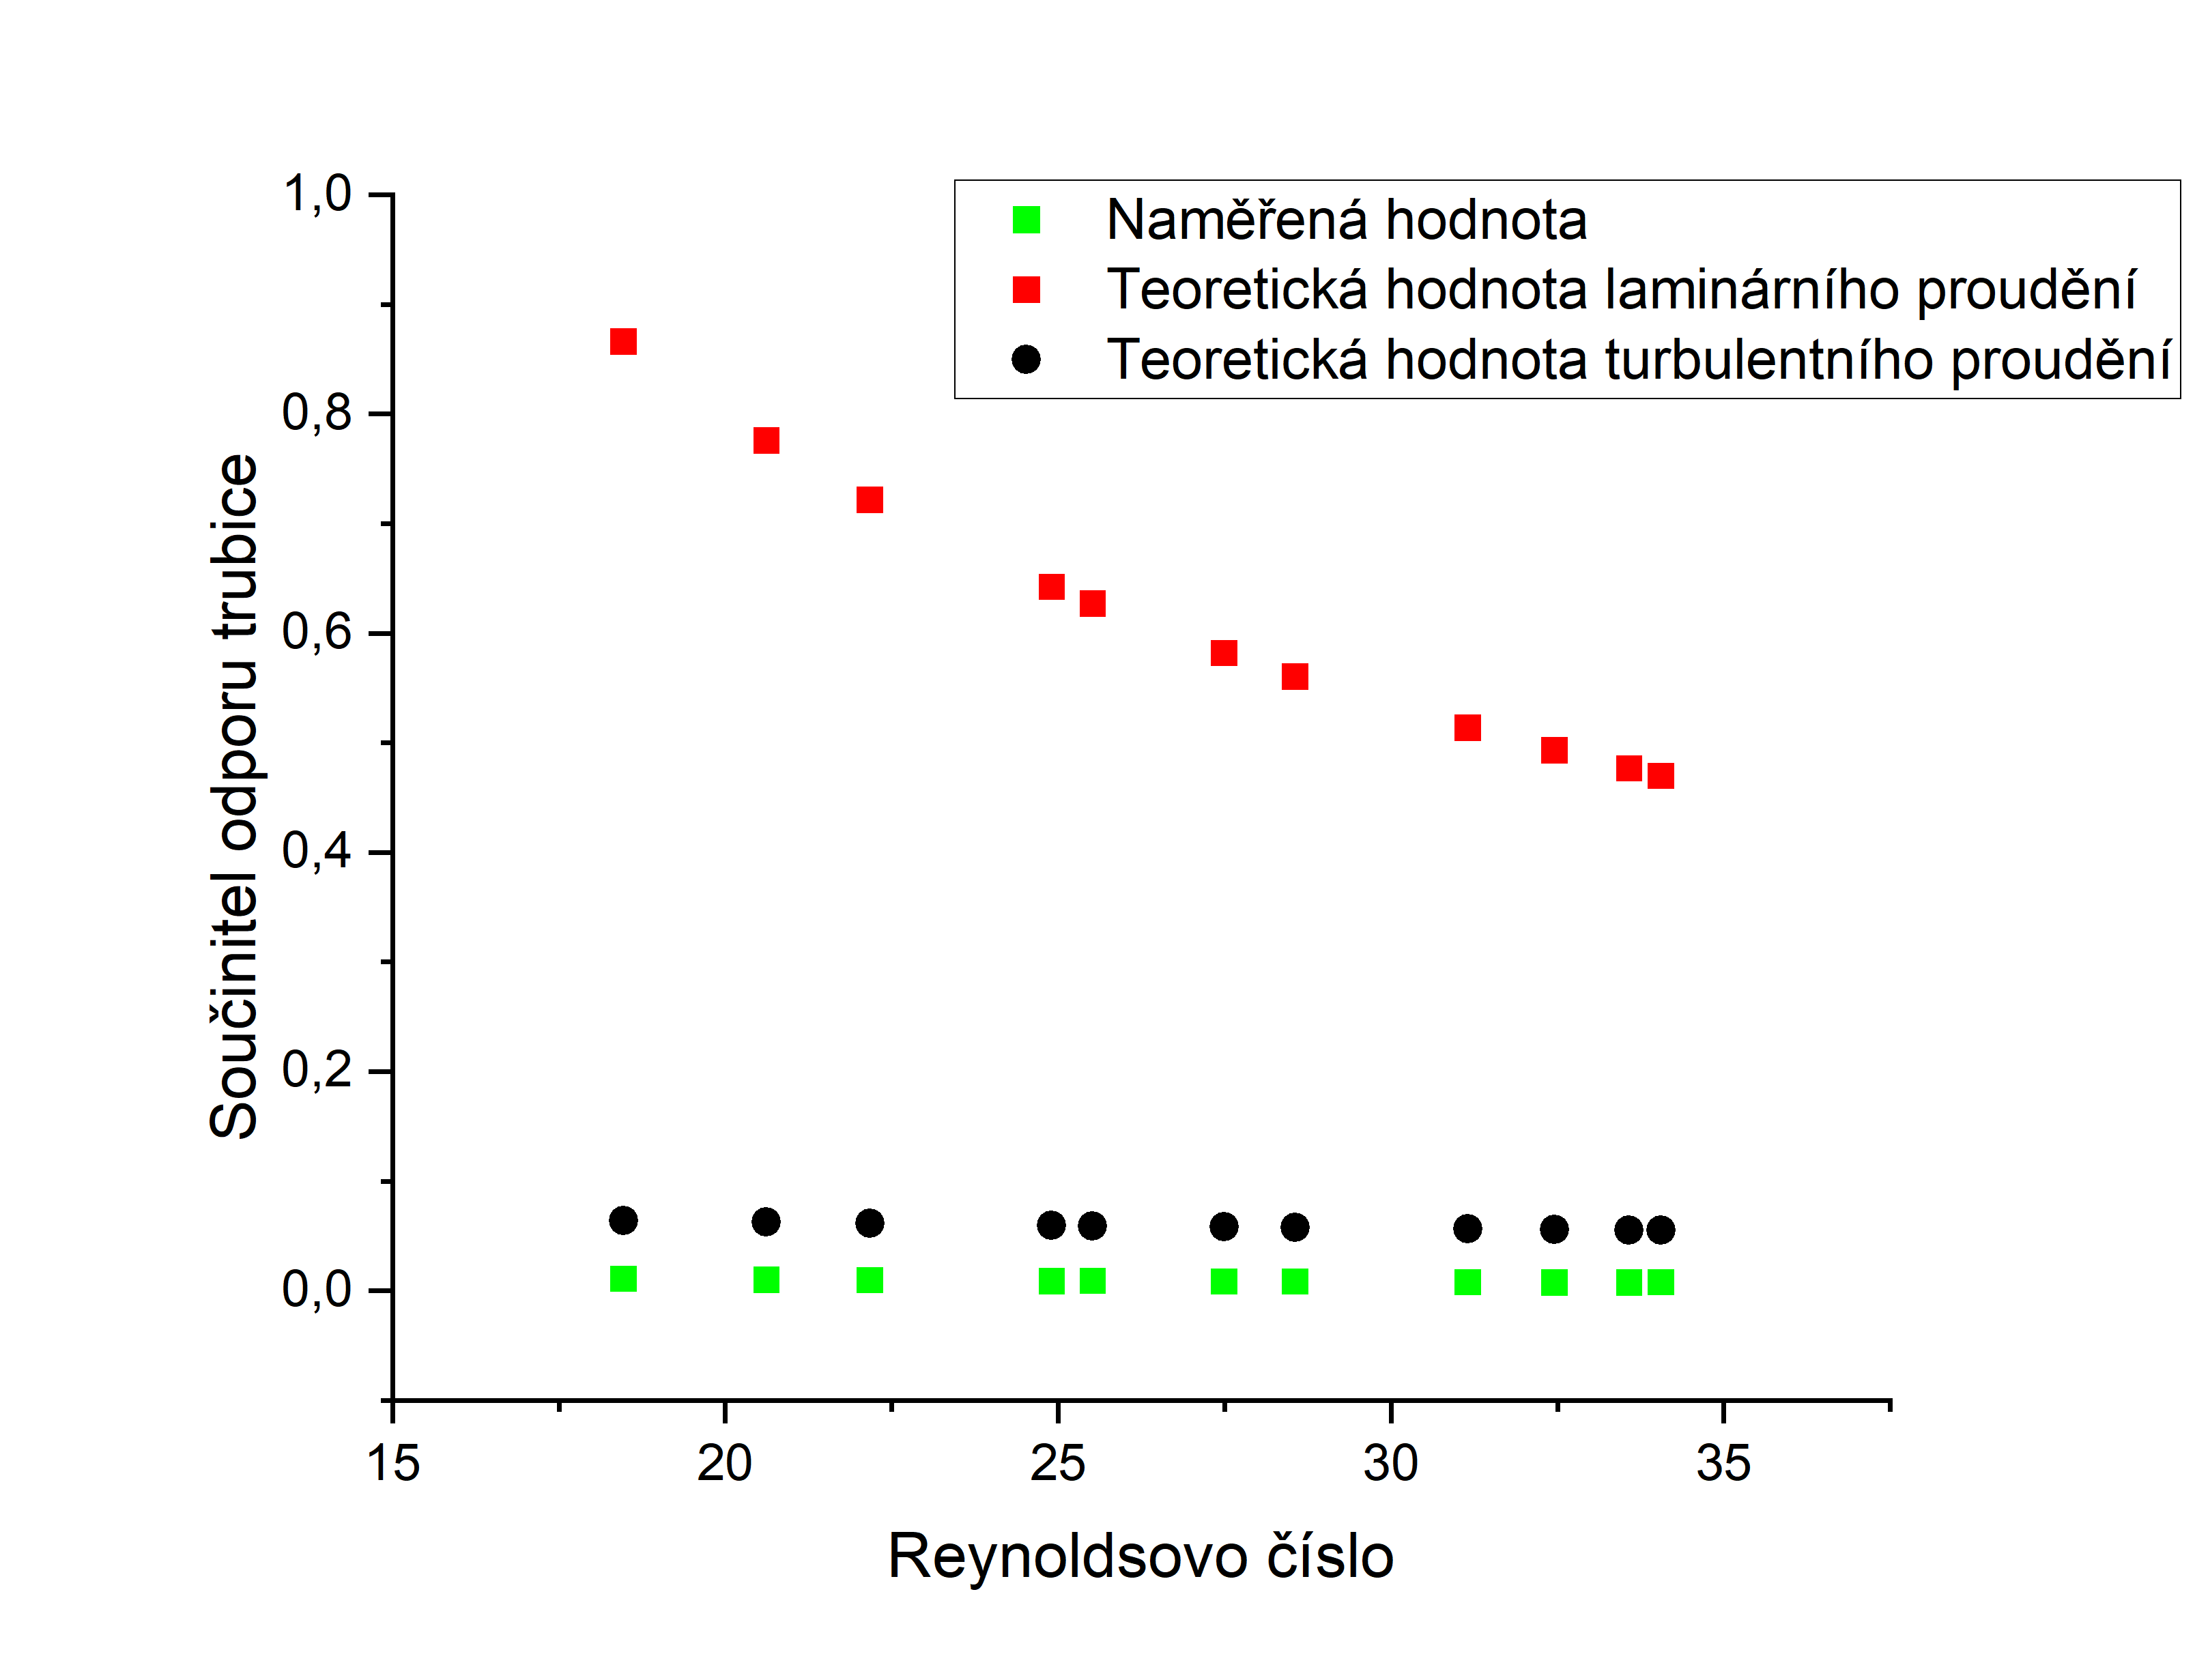
\includegraphics[width=0.6\linewidth]{01 - Studium proudění viskózní kapaliny trubicemi kruhového průřezu//Protokol//img/Re(k) B.png}
        \caption{Závislost součinitele odporu trubice B na Reynoldsově čísle}
        \label{fig:Re(k)) B}
    \end{figure}

    \begin{figure}[h]
        \centering
        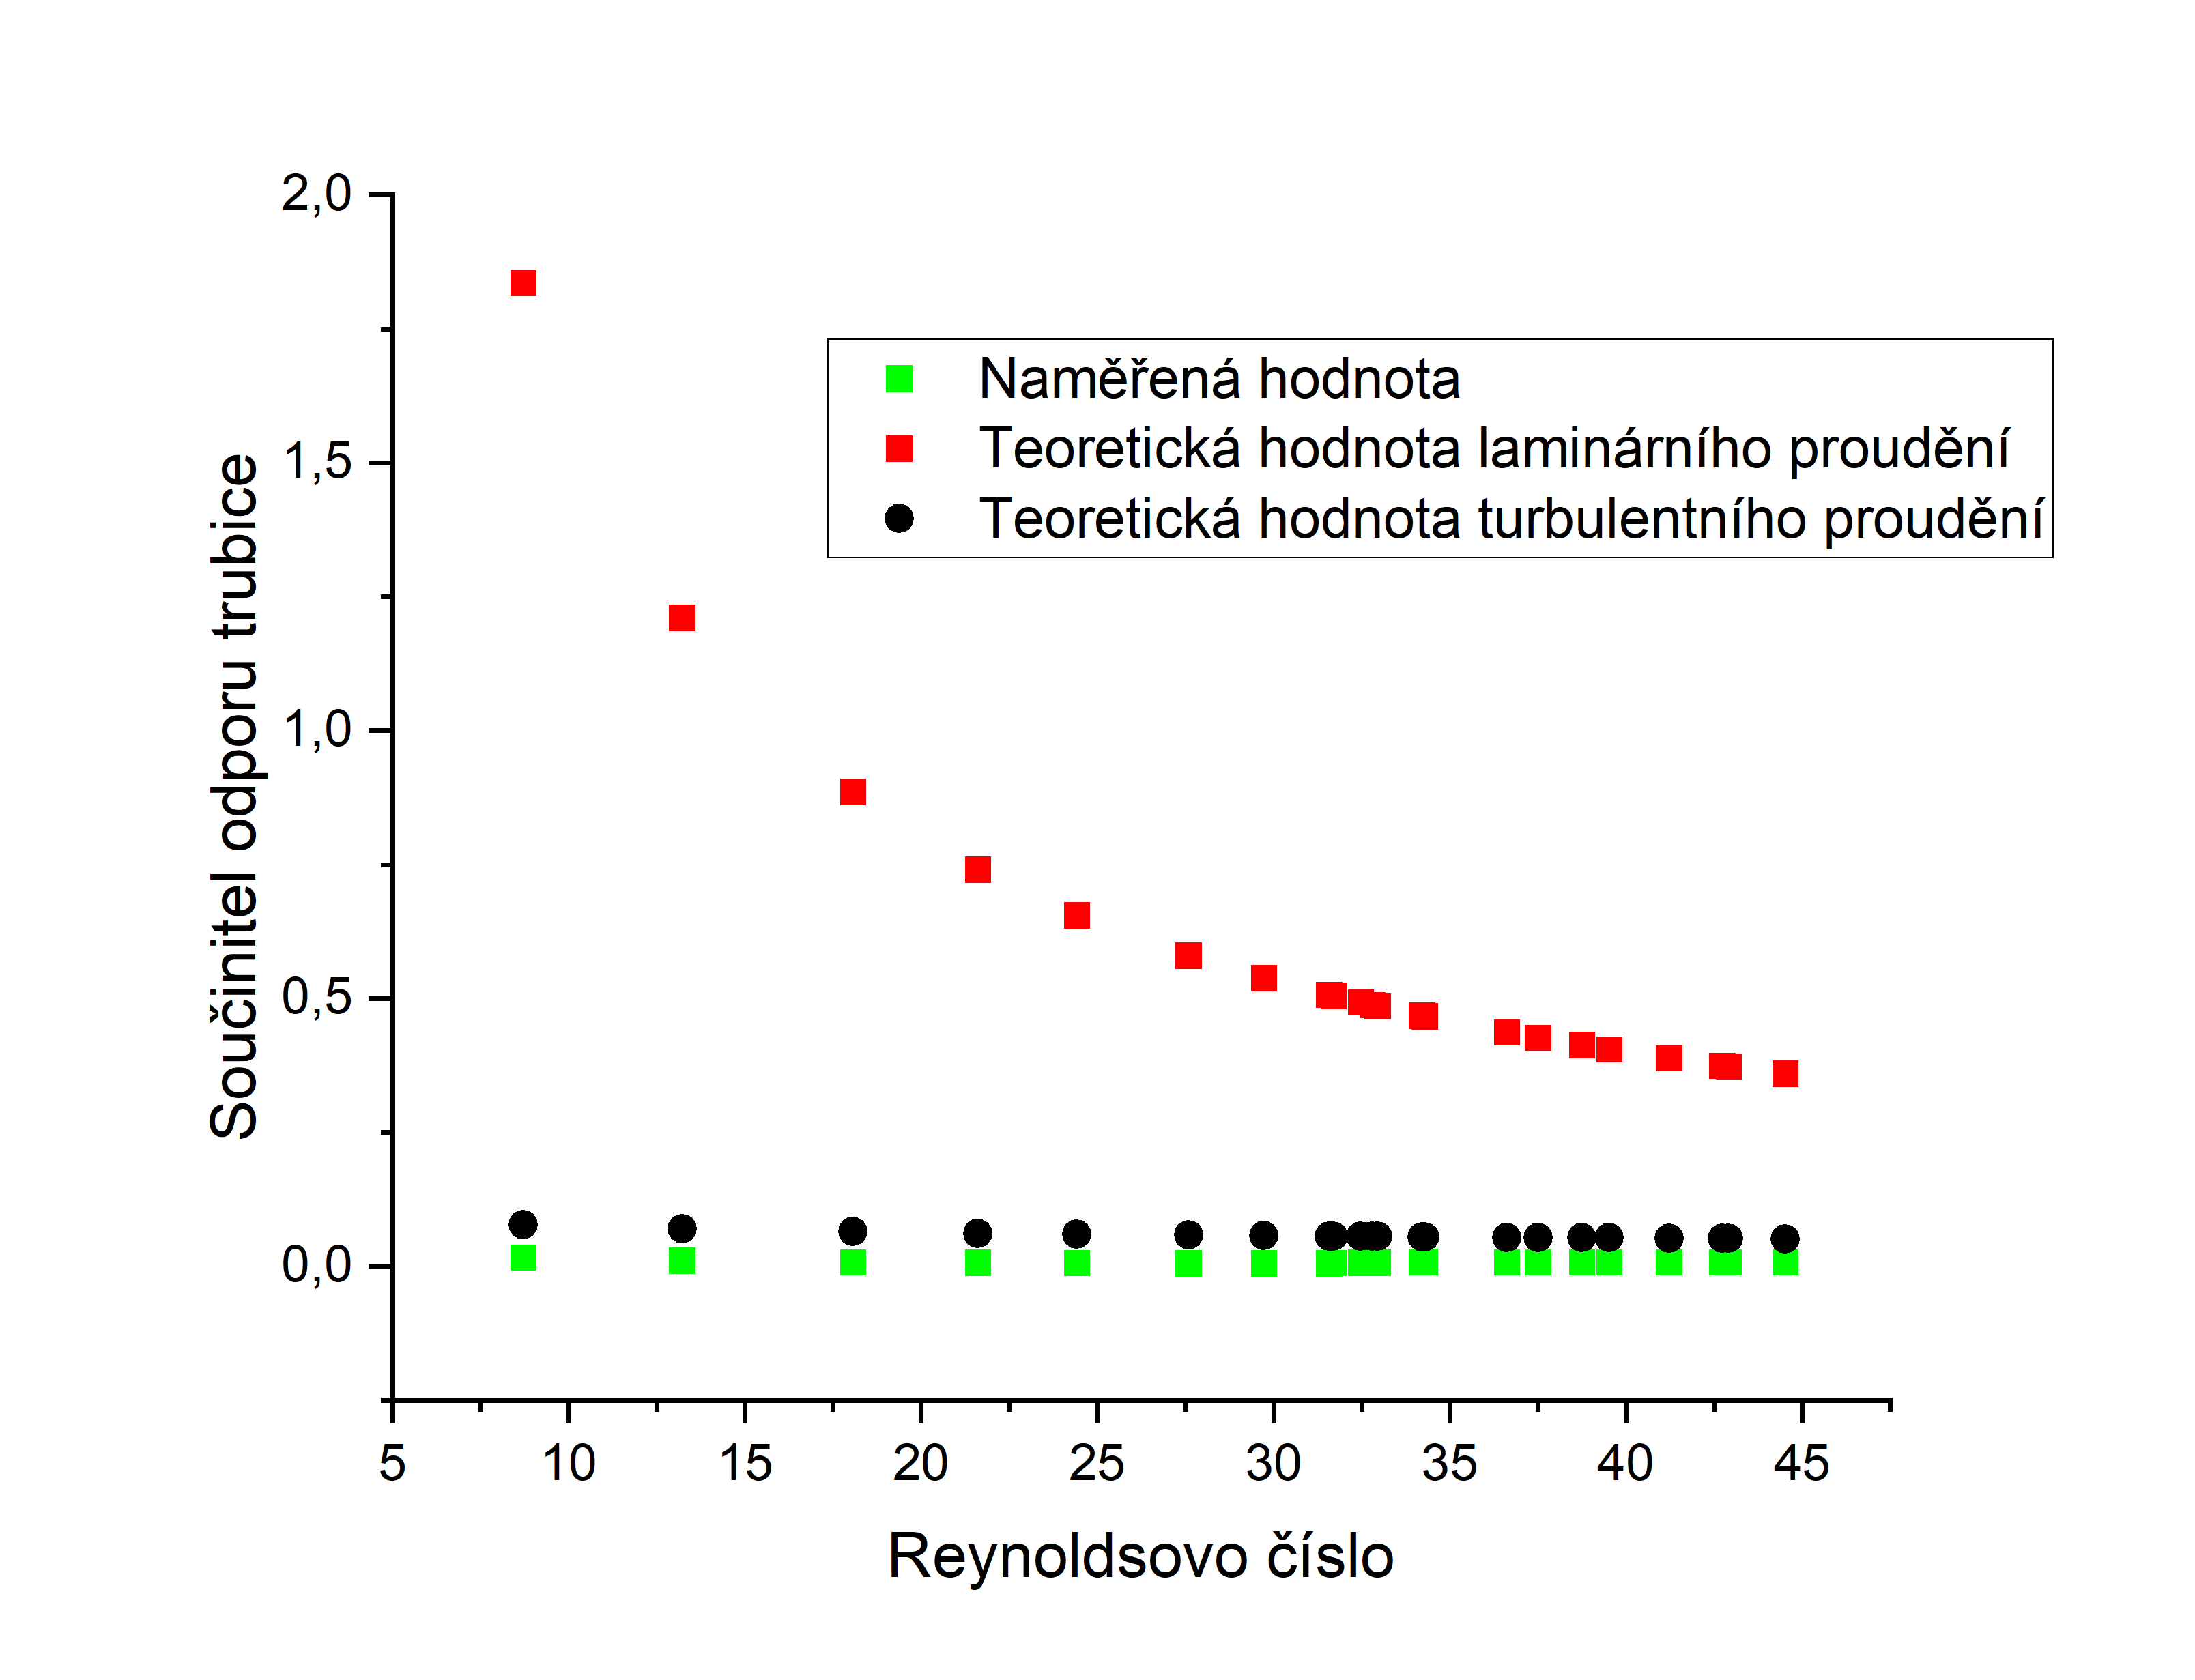
\includegraphics[width=0.6\linewidth]{01 - Studium proudění viskózní kapaliny trubicemi kruhového průřezu//Protokol//img/Re(k) C.png}
        \caption{Závislost součinitele odporu trubice C na Reynoldsově čísle}
        \label{fig:Re(k) C}
    \end{figure}
\newpage
    
% ----------------------------------------------------------------------
%  Diskuse výsledků
% ----------------------------------------------------------------------			
\section{Diskuse výsledků}

    Z obrázku \ref{fig:graf trubic} je možné vyčíst do jaké výšky manometru leží jednotlivé výsledky na přímce a tedy mají laminární průběh.

    Trubice A je ve všech měřených bodech laminární. To se shoduje i s pozorováním v průběhu měření. Na grafu je vidět bod s výškou 20 cm, který je jako jediný vzdálený od fitované přímky. Jedná se pravděpodobně o nepřesnost měření způsobená vysokou výškou hladiny vody v manometru, kde již může být zhoršená přesnost měření.

    V trubici B leží body na přímce do výšky 12 cm, což se také plně shoduje s pozorováním. Bod ve výšce 10 cm také pravděpodobně nese malou nepřesnost měření.

    V případě trubice C lineární regrese prochází celkem 7 body, což odpovídá do výšky 8 cm. Ve skutečnosti bylo pozorováno laminární chování (hladina vody v manometru neoscilovala) v oblasti s alespoň o 5 cm vyšší hladinou, než vychází z grafu. Bodů pro analýzu bylo změřeno dostatek, ale vylepšit tento experiment lze měřením objemu vody proteklou trubicí s vyšší přesností.

    Avšak i přes nižší přesnost měření u trubice C je nejistota přijatelná, jak vidíme na obrázku \ref{fig:graf trubic}. U trubic A a B je chyba měření tak malá, že ani nejsou na grafu vidět jednotlivé chybové úsečky.

    V porovnání vnitřních průměrů trubic změřených nepřesným plastovým posuvným měřidlem a vypočteným ze směrnice grafu rozdíl vyšel překvapivě nízký, téměř zanedbatelný. Plastové měřidlo již bylo lehce opotřebované a trubice nemusela mít ve všech směrech stejný průměr. Díky těmto vynikajícím výsledkům jsme ověřili, že takto zvolené směrnice přímek jsou vhodné dobře odpovídající realitě.

    U grafů závislosti součinitele odporu trubice na Reynoldsově čísle naměřené hodnoty spíše korelují s turbulentním prouděním.

% ----------------------------------------------------------------------
%  Závěr
% ----------------------------------------------------------------------
\section{Závěr}

    V tomto experimentu jsme úspěšně změřily závislosti objemových průtoků na úbytku statického tlaku všech třech trubic. Poté jsme sestrojili jednotlivé grafy a určili oblasti laminárního proudění. Jak ukazují výpočty, tyto oblasti byly vhodně zvoleny.

    Grafy závislosti k=k(Re) porovnávají teoretickou hodnotu laminárního a turbulentního proudění s hodnotou naměřenou.
